\header{
    \section{Au clair de la lune} \label{au-clair-de-la-lune}
    %
    
    \insertComment{Adaptation de la comptine datée de ~1790 et originaire d'Ile de France.}{}
    
    %L'air serait de J-B Lully, et l'histoire déjà connue en 1553 à Lyon.
}

\enluminure{4}{\href{https://www.youtube.com/watch?v=IYLTc3tGdzc}{A}}{u clair} de la lune,
\\Mon ami Pierrot,
\\Prête-moi ta plume,
\\Mon mari est sot.
\\Sa chandelle est morte,
\\Et manque de feu
\\Ouvre-moi ta porte,
\\Pour baiser un peu.
\dualcol{
\\\\Au clair de la lune, %2ème paragraphe
\\Pierrot répondit:
\\"Je garde ma plume,
\\Pour baiser Nini.
\\Va chez la voisine,
\\Elle aime s'amuser.
\\Elle est un peu gouine,
\\Elle a du doigté."
\\\\Mais chez la voisine
\\Y avait un monde fou
\\Des chambres aux cuisines
\\On baisait partout
\\Et sur la pelouse,
\\Des gens distingués,
\\Faisaient une partouze:
\\C'était follement gai.
\\\\Au clair de la lune,
\\J'entrais dans le jeu,
\\Entouré de plumes,
\\C'était merveilleux.
\\J'en pris une belle,
\\Sur un rayon d'or,
\\Ah quelle chandelle :
\\Je la sens encore.
\\\\Au clair de la lune, %Dernier paragraphe
\\Je fus au déduit,
\\Je pris toutes les plumes,
\\Ohlala quelle nuit !
\\Soufflées de la sorte,
\\Par le vent d'amour,
\\Les chandelles sont mortes,
\\Au lever du jour.\\
\begin{center}
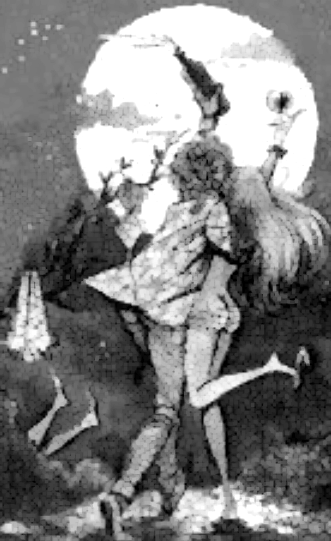
\includegraphics[width=0.3\textwidth]{images/lune2.png}
\end{center}
}

\breakpage